\documentclass[xcolor=pdftex,dvipsnames]{beamer}

\usepackage{amsmath}
\usepackage{amssymb}
\usepackage{comment}
\usepackage{textcomp}

\title{Microeconomic Theory --- ECON 323 503 \\ Chapter 4: Demand}
\author{Vikram Manjunath}
\institute{Texas A\&M University}
\setbeamertemplate{navigation symbols}{}
\setbeamertemplate{footline}{}
\usefonttheme{serif}
\begin{document}

\maketitle

\begin{frame}
\frametitle{Outline}
\begin{enumerate}[<+->]
\item Deriving demand curves: Where do the demand curves that we saw
  in Chapter 2 come from?
\item Effects of an increase in income: How does quantity demanded
  depend on income?
\item Effects of an increase in price:  How does quantity demanded
  depend on the price of a good?
\item Revealed preference: How do we figure out preferences from the
  choices that we observe?
\end{enumerate}
\end{frame}

\begin{frame}
\frametitle{Deriving Demand Curves}
We saw how a consumer chooses bundles $(q_1,q_2)$ for given prices
$(p_1,p_2)$ and income  ($Y$).

This describes a demand function for each good:
\[
\begin{array}
{rcl}
q_1 &=& D_1(p_1,p_2,Y)\\
q_2 &=& D_2(p_1,p_2,Y)\\
\end{array}
\]

\end{frame}

\begin{frame}
\frametitle{Demand functions for particular utility functions}
\begin{enumerate}
\item Perfect complements
\item Cobb-Douglas
\item Perfect substitutes
\item Quasilinear
\item Constant elasticity of substitution
\end{enumerate}
\end{frame}


\begin{frame}
\frametitle{Perfect complements}
\[
U(q_1,q_2) = \min\{q_1,q_2\}
\]
\uncover<2->{
You would only purchase the goods in equal proportion: you'd buy units
of the ``combined'' good. E.g. you wouldn't buy different numbers of
left and right shoes.}


\uncover<3->{
\bigskip The price of a combined good is $p_1+p_2$ per unit. 
}

\uncover<4->{
\bigskip If you spent all
your money ($Y$), you'd buy $\frac{Y}{p_1+p_2}$ units. So
\[
\begin{array}
{rcl}
D_1(p_1,p_2,Y) &=& \frac{Y}{p_1+p_2}\\\\
D_2(p_1,p_2,Y) &=& \frac{Y}{p_1+p_2}\\
\end{array}
\]}
\end{frame}

\begin{frame}
\frametitle{Demand curve for perfect complements}
Once we have the demand function for a good, we can draw the demand
curve.
\bigskip

\uncover<2->{
To get the demand curve for good 1, leave the price of good 2 ($p_2$)
and income ($Y$) fixed at say $p_2=3$ and $Y=9$
\[
D_1(p_1) = \frac{9}{p_1+3}
\]
}
\uncover<3->{

\begin{center}
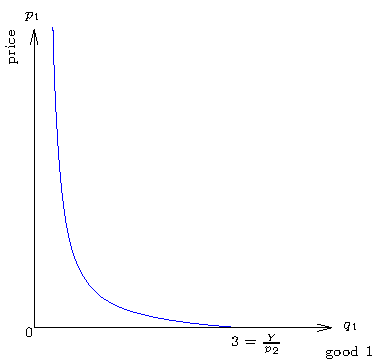
\includegraphics[scale=0.8]{pics/PerfCompDC}
\end{center}
}
\end{frame}

\begin{frame}
\frametitle{Cobb-Douglas}
\[
U(q_1,q_2) = q_1^aq_2^{1-a}
\]

\bigskip
\uncover<2->{
\[
\begin{array}{rcl}
D_1(p_1,p_2,Y)&=& \frac{aY}{p_1}\\\\
D_2(p_1,p_2,Y)&=& \frac{(1-a)Y}{p_2}\\\\
\end{array}
\]
}

\end{frame}
\begin{frame}
\frametitle{Demand curve for Cobb-Douglas utility}
Again, for fixed $a$,  $p_2$, and $Y$, we can find a demand curve.

\uncover<2->{
If $a=0.25$ and $Y = 10$, then 
\[
D_1(p_1) = \frac{2.5}{p_1}.
\]
}
\uncover<3->{
\begin{center}
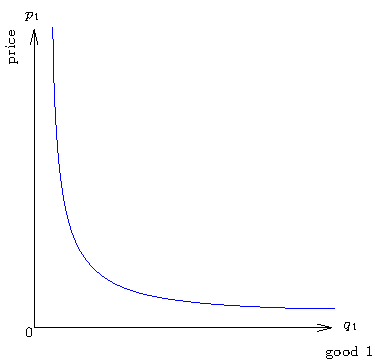
\includegraphics{pics/CDDC}
\end{center}
}
\end{frame}

\begin{frame}
\frametitle{Perfect substitutes}
\[
U(q_1,q_2) = q_1+q_2
\]

 \uncover<2->{If both goods have the same price you buy whatever. Otherwise, buy the
cheaper of the two.}
\bigskip


\uncover<3->{ If $p_1=p_2=p$
\[
D_1(p_1,p_2,Y) + D_2(p_1,p_2,Y) = \frac{Y}{p}
\]}

\uncover<4->{If $p_1<p_2$
\[
D_1(p_1,p_2,Y)  = \frac{Y}{p_1}\text{ and } D_2(p_1,p_2,Y)=0
\]}

\uncover<5->{If $p_1>p_2$
\[
D_1(p_1,p_2,Y)  = 0\text{ and } D_2(p_1,p_2,Y)=\frac{Y}{p_2}
\]}
\end{frame}

\begin{frame}
\frametitle{Demand curve for perfect substitutes}
Again, for fixed $p_2$ and $Y$, we can find a demand curve.

\uncover<2->{If $p_2=3$ and  $Y = 12$, then 
\[
D_1(p_1) = \left\{\begin{array}{l} \text{any }q_1\text{ between 0 and
    }\frac{12}{p_1}\text{ if } p_1= 3\\\\
0 \text{ if }  p_1>3\\\\\frac{12}{p_1}\text{ if }p_1<3
\end{array}\right.
\]}

\uncover<3->{\begin{center}
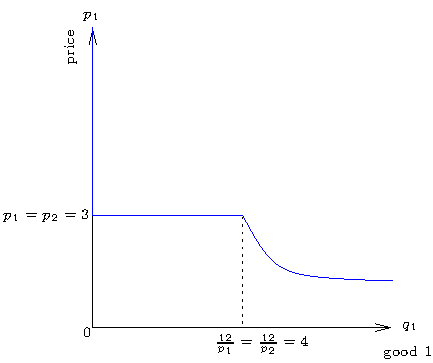
\includegraphics[scale=0.7]{pics/PerfSubDC}
\end{center}}
\end{frame}

\begin{frame}
\frametitle{Quasilinear}
This will depend on the exact utility function. Let's take an example:
\[
U(q_1,q_2) = a\sqrt{q_1} + q_2
\]

\uncover<2->{There are two cases.}
\bigskip

\uncover<3->{Interior solution if $Y>\frac{a^2p_2}{4p_1}$
\[
\begin{array}{rcl}
D_1(p_1,p_2,Y)&=& \left(\frac{ap_2}{2p_1}\right)^2\\\\
D_2(p_1,p_2,Y)&=& \frac{Y}{p_2} - \frac{a^2p_2}{4p_1}
\end{array}
\]}
\uncover<4->{
Corner solution if  $Y\leq\frac{a^2p_2}{4p_1}$
\[
\begin{array}{rcl}
D_1(p_1,p_2,Y)&=& \frac{Y}{p_2}\\\\
D_2(p_1,p_2,Y)&=& 0
\end{array}
\]
}
\end{frame}


\begin{frame}
\frametitle{Constant elasticity of substitution (CES)}
\[U(q_1,q_2) = (q_1^\rho+q_2^\rho)^{\frac{1}{\rho}}
\]

Assuming $0<\rho<1$ and letting $\sigma=\frac{1}{\rho-1},$
\[
 \begin{array}{rcl}
D_1(p_1,p_2,Y)&=& \frac{Yp_1^\sigma}{p_1^{\sigma+1} + p_2^{\sigma_1}}\\\\
D_2(p_1,p_2,Y)&=& \frac{Yp_2^\sigma}{p_1^{\sigma+1} + p_2^{\sigma_1}}\\\\
\end{array}
\]

\end{frame}


\begin{frame}
\frametitle{Deriving demand curves graphically}
What happens as we hold everything fixed ($p_2=1$ and $Y=20$) but vary
$p_1$?
\uncover<2->{\begin{center}
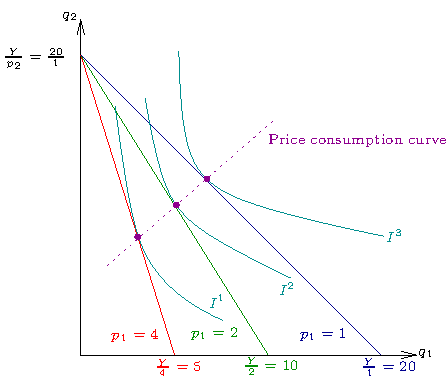
\includegraphics{pics/DemandCurveDeriv}
\end{center}

}
\end{frame}
\begin{frame}\begin{center}
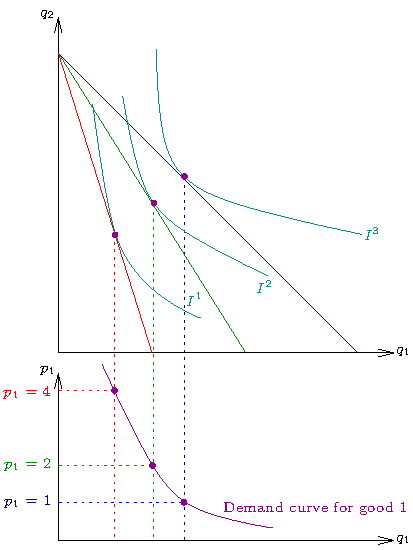
\includegraphics[scale=0.9]{pics/DemandCurveDeriv2}
\end{center}\end{frame}



\begin{frame}\frametitle{Textbook exercise 1.5}

\[
U(q_1,q_2) = 2\sqrt{q_1} + q_2
\]What are the demand functions for the two goods?

\bigskip
\uncover<2->{
What we want to find are $D_1(p_1,p_2,Y)$ and  $D_2(p_1,p_2,Y)$.
\bigskip}

\uncover<3->{
Need to solve \[
\begin{array}{c}\displaystyle\max_{q_1q_2} 2\sqrt{q_1} + q_2\\
\text{s.t. }p_1q_1+p_2q_2 = Y.\end{array}
\]
}
\uncover<4->{
Substituting $q_2=\frac{Y-p_1q_1}{p_2}$,
\[\max_{q_1}\ 2\sqrt{q_1} + \frac{Y-p_1q_1}{p_2}.
\]
}

\end{frame}
\begin{frame}
\frametitle{Textbook exercise 1.5}
First order condition:
\[
2\frac{1}{2}\frac{1}{\sqrt{q_1}} - \frac{p_1}{p_2} = 0
\]
\uncover<2->{
\[
\frac{1}{\sqrt{q_1}} =\frac{p_1}{p_2}
\]
}
\uncover<3->{
\[
\sqrt{q_1} =\frac{p_2}{p_1}
\]
}
\uncover<4->{
\[q_1 = \left(\frac{p_2}{p_1}\right)^2\]
}
\uncover<5->{
So, $D_1(p_1,p_2,Y) = \left(\frac{p_2}{p_1}\right)^2$
}
\end{frame}
\begin{frame}\frametitle{Textbook exercise 1.5}

Substituting back to solve for $q_2$:
\[
\begin{array}{rl}q_2 &= \frac{Y-p_1q_1}{p_2}\\\\&\uncover<2->{ = \frac{Y}{p_2} - \frac{p_1}{p_2}q_1 \\\\}\uncover<3->{&=
\frac{Y}{p_2} - \frac{p_1}{p_2}\left(\frac{p_2}{p_1}\right)^2  \\\\}\uncover<4->{&=
\frac{Y}{p_2} -  \frac{p_2}{p_1}}\end{array}
\]
\uncover<5->{
So, $D_2(p_1,p_2,Y) = \frac{Y}{p_2} -  \frac{p_2}{p_1}$.}
\end{frame}

\begin{frame}
\frametitle{Effects of an increase in income}
If, holding everything constant, consumer income increases, we argued
before that the demand curve ``shifts.'' 

\uncover<2->{
Let's analyze this more closely.
}

\bigskip
\uncover<3->{What happens to the consumer's opportunity set? It gets bigger. The
budget line shifts outward.
}

\uncover<4->{
\bigskip
Suppose that $p_1 = p_2 = 1$.
\begin{center}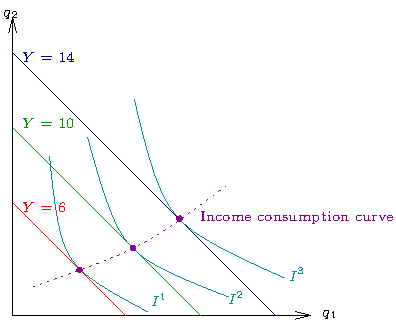
\includegraphics[scale=0.8]{pics/IncomeExp}\end{center}
}
\end{frame}
\begin{frame}
\begin{center}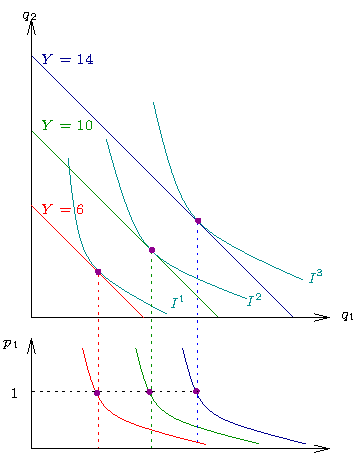
\includegraphics{pics/IncomeExp1}\end{center}
\end{frame}
\begin{frame}\frametitle{The Engel curve}
\begin{center}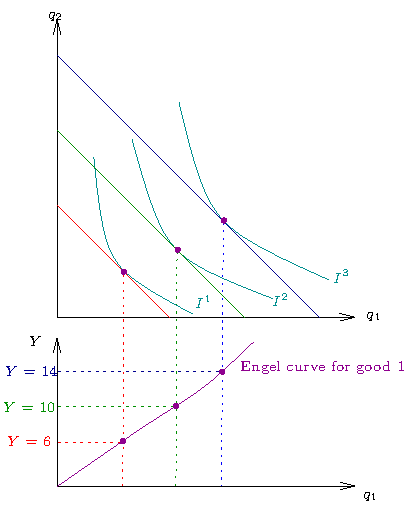
\includegraphics{pics/Engel}\end{center}
\end{frame}


\begin{frame}\frametitle{Income elasticity}
How does demand respond to changes in income?
\bigskip

\uncover<2->{Useful for firms to know the impact of things like an income tax.}



\uncover<3->{\[
\xi = \frac{\text{\% change in quantity demanded}}{\text{\% change in
      income}}=\frac{\delta Q}{\delta Y}\frac{Y}{Q}
\]}
\end{frame}

\begin{frame}\frametitle{Interpreting $\xi$}
When  $\xi = 1$, if income increases by  1\% the quantity demanded
increases by 1\%.

\bigskip
\uncover<2->{Is it possible for $\xi < 0$?}

\bigskip
\uncover<3->{ Yes, for \emph{inferior goods}. As income rises, you consume
 \emph{less} of such goods. Examples: fastfood, pirated goods.}

\bigskip
\uncover<4->{Good for which $\xi>0$: \emph{normal goods}.}

\bigskip
\uncover<5->{What if $\xi>1$?}

\bigskip
\uncover<6->{Your consumption of such a good grows \emph{faster} than your
income. \emph{Luxury goods}.}
\bigskip

\uncover<7->{If $0\leq \xi\leq 1$ the good is called a \emph{necessity}.}
\end{frame}

\begin{frame}\frametitle{Income consumption curves and income
    elasticities}
The shape of the ICC tells us if goods are normal or inferior.
\begin{center}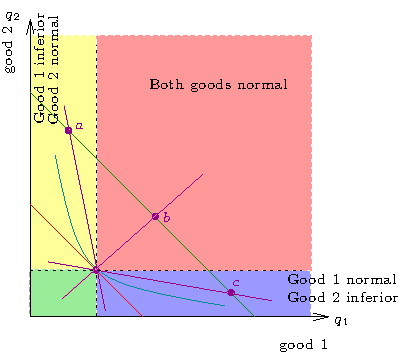
\includegraphics{pics/InfNormal}
\end{center}
\uncover<2->{This picture shows us that both goods can't be inferior: there's
always at least one normal good.}
\end{frame}


\begin{frame}
\frametitle{There's always a normal good}
If there are $n$ goods, at least one of them has to be normal:

\bigskip
\uncover<2->{Budget constraint:
\[
p_1q_1 + p_2 q_2 + \dots +p_nq_n = Y.
\]}
\uncover<3->{
Differentiating with respect to $Y$:
\[
p_1\frac{dq_1}{dY} + p_2\frac{dq_2}{dY} + \dots +p_n\frac{dq_n}{dY}
= 1.
\]}
\uncover<4->{Multiply and divide each term by $q_iY$:
\[\frac{p_1q_1}{Y}\frac{dq_1}{dY} \frac{Y}{q_1}+ \frac{p_2q_2}{Y} \frac{dq_2}{dY}\frac{Y}{q_2} + \dots +\frac{p_nq_n}{Y}\frac{dq_n}{dY}\frac{Y}{q_n}
= 1.
\]}
\uncover<5->{Since $\xi_i = \frac{dq_1}{dY} \frac{Y}{q_1}$,
\[
\theta_1 \xi_1 + \theta_2 \xi_2 + \dots+\theta_n \xi_n =1
\]
where $\theta_i=\frac{p_iq_i}{Y}$.}
\bigskip

\uncover<6->{Since the $\theta$s sum to 1, there has to be at least one $\xi$ that
is positive.}
\end{frame}
\begin{frame}
\frametitle{Textbook exercise 2.4}
\[
U(q_1,q_2) = q_1^{0.6}q_2^{0.4}
\]
Find the equation of the Engel curve for good 2.
\bigskip

\uncover<2->{What we want is $Y$ as a function of $q_2$.\bigskip
}

\uncover<3->{Since this is a Cobb-Douglas utility function, we know
  that
\[q_2 = \frac{(1-a)Y}{p_2} = \frac{0.4Y}{p_2}.
\]}

\uncover<4->{So
\[
Y=\frac{p_2q_2}{0.4}
\]
}
\uncover<5->{This should be easy for you to graph.}

\end{frame}
\begin{frame}
\frametitle{Effects of a price increase}
The effect of a price increase has two parts:
\begin{enumerate}[<+->]
\item Income effect: if the price goes up, your income is \emph{worth} less.
\item Substitution effect: if the price goes up, you switch to buying
  other goods.
\end{enumerate}
\uncover<3->{
Knowing how the overall effect is split between these two allows us to
better forecast the effects of policies.}
\end{frame}

\begin{frame}
\frametitle{Income and substitution effects with a normal good}
Recall that an increase in $p_1$ causes the budget line to rotate
inwards.\bigskip

\uncover<2->{Start with $p_1=0.5$ and $p_2=1$. If the price of good 1 increases to $p_1'=1$, then
the budget line rotates (from $L^1$ to $L^2$).
\bigskip}

\uncover<3->{It is twice as steep: 
\[\begin{array}{l}\text{Slope of } L^1 = -\frac{p_1}{p_2} =
-\frac{0.5}{1} = -0.5\\\\
\text{Slope of } L^2 = -\frac{p_1'}{p_2} = 
-\frac{1}{1} = -1
\end{array}
\]}

\end{frame}
\begin{frame}\frametitle{The budget line rotates}
If $Y=30$,
\begin{center}
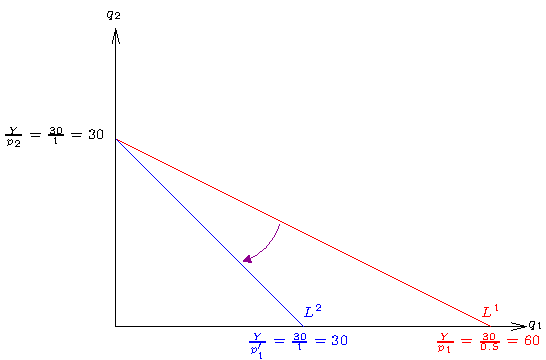
\includegraphics{pics/BudgetRotate}
\end{center}
\end{frame}

\begin{frame}
\frametitle{Income and substitution effects with a normal good}
\[
U(q_1,q_2) = q_1^{0.4}q_2^{0.6}
\]

\uncover<2->{Remember that demand is
\[
\begin{array}
{rcl}
q_1 &=& 0.4\frac{Y}{p_1} = 0.4\frac{30}{0.5} = 24\\\\
q_2 &=& 0.6\frac{Y}{p_2} = 0.6\frac{30}{1} = 18
\end{array}
\]}
\uncover<3->{
What happens when the price of good 1 rises?
\[
\begin{array}
{rcl}
q_1'&=& 0.4\frac{Y}{p_1'} = 0.4\frac{30}{1} = 12\\\\
q_2' &=& 0.6\frac{Y}{p_2} = 0.6\frac{30}{1} = 18
\end{array}
\]}
\uncover<4->{Price: $0.5\to 1$

Quantity demanded: $24\to 12$.
}
\end{frame}


\begin{frame}
\frametitle{Income and substitution effects with a normal good}
\begin{center}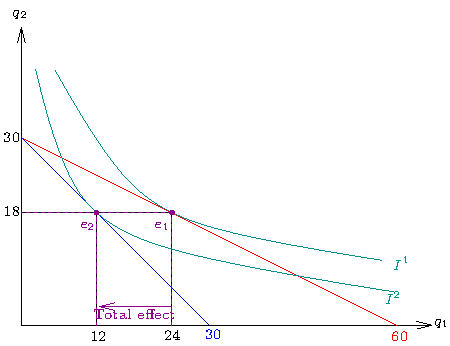
\includegraphics{pics/NormalIncSubEffect1}
\end{center}

We can split this into the two parts.
\end{frame}

\begin{frame}
\frametitle{Income and substitution effects with a normal good}
\begin{center}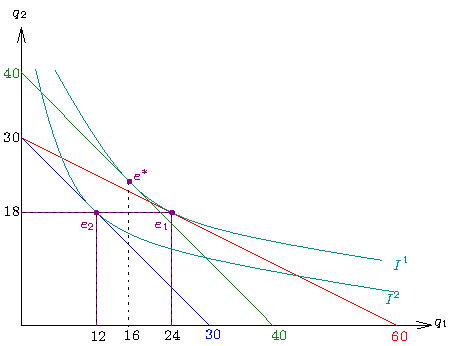
\includegraphics{pics/NormalIncSubEffect2}
\end{center}

Increase income to keep consumer on the same IC.
\end{frame}

\begin{frame}
\frametitle{Income and substitution effects with a normal good}
\begin{center}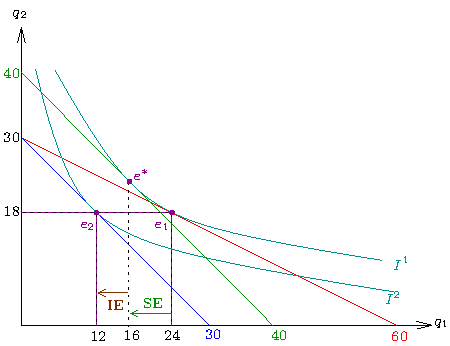
\includegraphics{pics/NormalIncSubEffect3}
\end{center}

This tells us how to split the total effect.
\end{frame}

\begin{frame}\frametitle{How'd we figure out how much to increase
    income?}
At original prices:
\[U_1(q_1,q_2)=24^{0.4}\times 18^{0.6}=(0.8\times 30)^{0.4}(0.6\times
30)^{0.6} = 30\times 0.8^{0.40}6^{0.6}.\]

\uncover<2->{If income is $Y$, demand at new price: $q_1^*=0.4\frac{Y}{p_1'}=0.4Y$
and $q_2^*=0.6\frac{Y}{1}=0.6Y$. 
\bigskip}

\uncover<3->{So at income $Y$ with new prices:
\[
U(q_1^*,q_2^*)= (0.4 Y)^{0.4}(0.6Y)^{0.6} = Y0.4^{0.4}0.6^{0.6}.
\] 
}
\uncover<4->{If utility is equal at the new income/prices to what it was
at old income/prices:
\[
30\times 0.8^{0.40}6^{0.6} = Y0.4^{0.4}0.6^{0.6}.
\]}
\uncover<5->{Solving this, $Y\approx 40$.}
\end{frame}

\begin{frame}
\frametitle{Income and substitution effects with a normal good}

\[
\textit{Total effect} = \textit{substitution effect} + \textit{income effect}
\]

\uncover<2->{Substitution effect causes you to move along your indifference curve:
remember that the slope changes as we move.\bigskip
}

\uncover<3->{Income effect causes you to move down to a lower indifference
curve. For \emph{normal goods}, this means that you consume less as the price
rises.}
\bigskip

\end{frame}

\begin{frame}
\frametitle{Income and substitution effects with an inferior good}
 For \emph{inferior goods} the income effect is in the opposite direction.
\bigskip

\uncover<2->{
For most inferior goods, substitution effect $>$ income effect.}
\bigskip

\uncover<3->{In that case, total effect is that an increase in price leads to a
decrease in quantity demanded, confirming the law of demand.\bigskip}

\uncover<4->{A (almost exclusively) theoretical alternative: \emph{Giffen
  goods}.\bigskip}



\uncover<5->{These violate the law of demand. Since substitution effect $<$ income
effect, increase in price increases demand. \bigskip}

\uncover<6->{Law of demand is an empirical observation. There are hardly any
examples of real world Giffen goods.}

\end{frame}




\begin{frame}
\frametitle{Compensated demand}

Typical  (\emph{Marshallian or uncompensated demand}) demand curve:
how quantity demanded varies as price changes.

\bigskip\uncover<2->{
\emph{Hicksian or compensated demand} curve: how quantity demand varies as price
changes \emph{and} consumer is given enough income to stay on the same
IC.}
\bigskip

\uncover<3->{Uncompensated demand depends only on prices and income:
$D_1(p_1,p_2,Y)$.\bigskip}

\uncover<4->{Compensated demand depends on utility level rather than income:
$H_1(p_1,p_2,\overline U)$.}

\bigskip
\uncover<5->{Cannot observe compensated demand: we don't know people's utility functions.}
\end{frame}

\begin{frame}\frametitle{Graphing the compensated demand curve }
\begin{center}
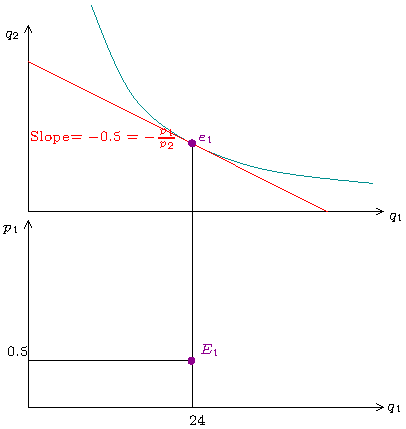
\includegraphics{pics/CompensatedDemand}
\end{center}


\end{frame}
\begin{frame}\frametitle{Graphing the compensated demand curve }
\begin{center}
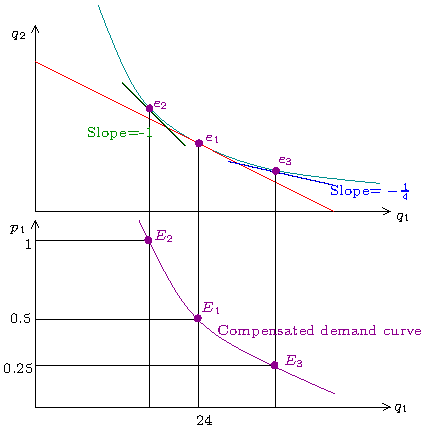
\includegraphics{pics/CompensatedDemand2}
\end{center}


\end{frame}



\begin{frame}\frametitle{Graphing the compensated demand curve }
\begin{center}
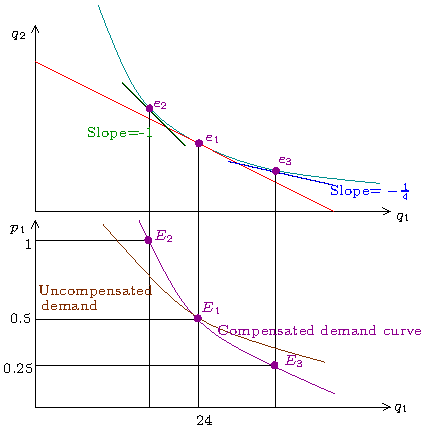
\includegraphics{pics/CompensatedDemand3}
\end{center}


\end{frame}

\begin{frame}\frametitle{The compensated demand curve }
The uncompensated demand curve crosses the compensated demand curve at
$E_1$: at the price $p_1=0.5$ both compensated and uncompensated
demand are the same (24). 
\bigskip

\uncover<2->{Don't need to compensate at that price, since that's our reference
point.
\bigskip}

\uncover<3->{Why is compensated demand curve steeper?
\bigskip}

\uncover<4->{It's only reflects the substitution effect. The total change is bigger due
to the income effect.}



\end{frame}





\begin{frame}
\frametitle{Cost minimization}
Target utility: $\overline U$
\bigskip

Prices: $p_1, p_2$
\bigskip

\uncover<2->{Expenditure at  $(q_1,q_2)$: $E= p_1q_1+p_2q_2$.}
\bigskip


\uncover<3->{You want to get to $\overline U$ as cheaply as possible:
\[
\begin{array}{c}\displaystyle\min_{q_1,q_2}p1q_1 + p_2q_2\\\\
\text{s.t. }U(q_1,q_2) = \overline U
\end{array}
\]}


\uncover<4->{This minimum value is the lowest income level at which you can get to
utility level $\overline U$: $E(p_1,p_2,\overline U)$.}
\end{frame}


\begin{frame}
\frametitle{Cost minimization}
\begin{center}
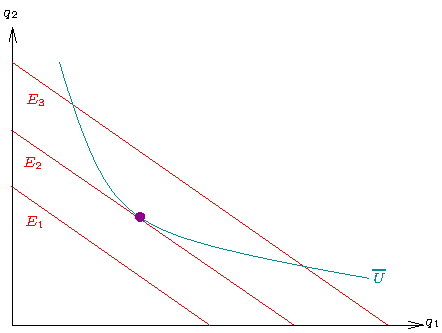
\includegraphics{pics/CostMin}
\end{center}
\end{frame}



\begin{frame}
\frametitle{Deriving compensated demand}
Use \emph{expenditure function} to derive compensated demand:

\[
\frac{\delta E}{\delta p_1}= H(p_1,p_2,\overline U) = q_1.
\]


\uncover<2->{This is \emph{Shephard's Lemma}. We won't prove it.}


\end{frame}
\begin{frame}
\frametitle{Textbook exercise 3.11}
\[
U(q_1,q_2)=q_1+2q_2
\]
What is the compensated demand function for good 1?

\uncover<2->{\bigskip
Step 1: Find the expenditure function:
\[
\begin{array}{rcc}E(p_1,p_2,\overline U) &=&
  \displaystyle\min_{q_1,q_2} p_1q_1 + p_2q_2\\&& \text{s.t. }q_1+2q_2
  = \overline U\end{array}
\]}
\uncover<3->{If $p_2 < 2p_1$ buy only good 2. Otherwise buy only good 1.
\bigskip}

\uncover<4->{If you buy only good 2, you need $\frac{\overline U}{2}$ units of
it. That costs $\frac{\overline U}{2}p_2$.\bigskip}

\uncover<5->{If you buy only good 1, you need $\overline U$ units of it. That costs
$\overline U p_1$.\bigskip}

\uncover<6->{So 
\[
E(p_1,p_2,\overline U) = \left\{
\begin{array}{l}
\frac{\overline U}{2}p_2 \text{ if }p_1>\frac{p_2}{2}\\\\
\overline Up_1\text{ if }p_1 \leq \frac{p_2}{2}
\end{array}
\right.
\]
}

\end{frame}

\begin{frame}
\frametitle{Textbook exercise 3.11}
Step 2: Differentiate the expenditure function
\[
H(p_1,p_2,\overline U) = \frac{\delta E}{\delta p_1}=\left\{\begin{array}{l}
0 \text{ if }p_1>\frac{p_2}{2} \\\\
\overline U\text{ if } p_1\leq\frac{p_2}{2} \\\\
\end{array}\right.
\]

\end{frame}




\begin{frame}\frametitle{The Slutsky equation}
\emph{Pure substitution elasticity of demand:}
\[
\varepsilon^*=\frac{\text{\% change in compensated demand}}{\text{\%
    change in price}} = \frac{\delta H}{\delta p_1}\frac{p_1}{H}
\] Describes the substitution effect.

\bigskip
\uncover<2->{Income effect is 
\\$\theta\xi=$ (share of income spent on the
good$)\times($income elasticity).
\bigskip}



\uncover<3->{\emph{Slutsky equation:}
\[
\underset{\text{\text{total effect}}}\varepsilon= \underset{\text{substitution
  effect}}{\varepsilon^*} +\underset{\text{income effect}}{(- \theta\xi)}
\]}
\end{frame}

\begin{frame}\frametitle{Revealed preference}
Can we infer a consumer's preferences if we observe the choices he
makes?

\uncover<2->{\bigskip This is what revealed preference is.}

\uncover<3->{\bigskip Assumption: consumers maximize utility subject to a budget
constraint.}

\bigskip
\uncover<4->{See what a consumer picks at various budgets and use this to back out
his preferences.}
\end{frame}

\begin{frame}
\frametitle{Backing out preferences}
\begin{center}
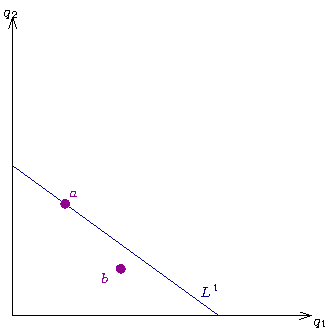
\includegraphics{pics/RevPref1}
\end{center}
You could have had $b$ but you picked $a$. So $a$ is \emph{revealed
  preferred to }$b$.
\end{frame}

\begin{frame}
\frametitle{Backing out preferences}
\begin{center}
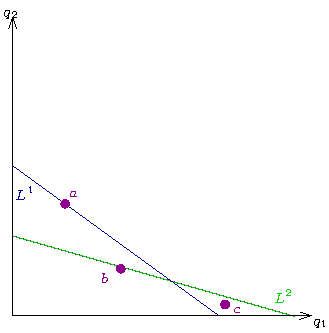
\includegraphics{pics/RevPref2}
\end{center}
If you had already revealed that you prefer $b$ to $c$, then you now
have revealed that you prefer $a$ to $c$ as well.
\end{frame}


\begin{frame}
\frametitle{Backing out preferences}
\begin{center}
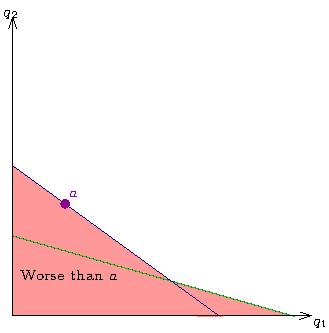
\includegraphics{pics/RevPref3}
\end{center}
This reasoning would tell us that you prefer $a$ to every bundle in
the shaded area.
\end{frame}

\begin{frame}
\frametitle{Backing out preferences}
\begin{center}
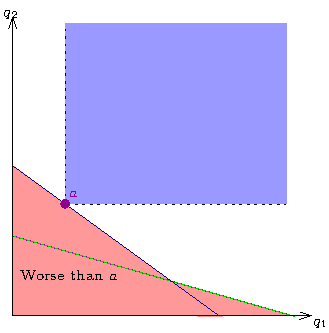
\includegraphics{pics/RevPref4}
\end{center}
Since preferences are monotonic, any bundle that has more of each good
is better than $a$.




\end{frame}

\begin{frame}
\frametitle{Backing out preferences}
\begin{center}
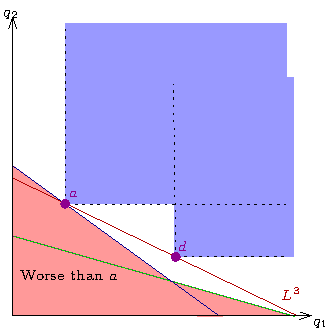
\includegraphics{pics/RevPref5}
\end{center}
If you pick $d$ when you could have $a$, then you reveal that $d$ is
preferred to $a$. Anything better than $d$ is also better than $a$.
\end{frame}


\begin{frame}
\frametitle{Backing out preferences}
\begin{center}
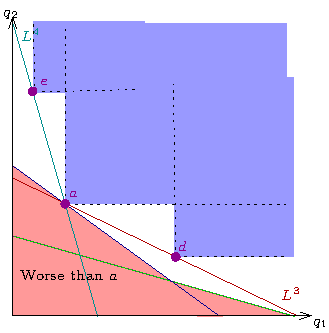
\includegraphics{pics/RevPref6}
\end{center}
You could similarly reveal that you prefer $e$ to $a$. \\
And so on.
\end{frame}

\begin{frame}
\frametitle{Backing out preferences}
\begin{center}
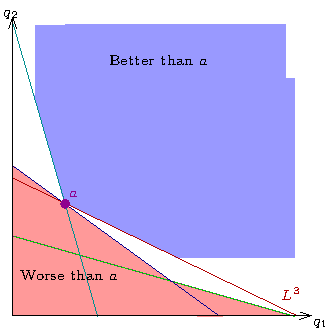
\includegraphics{pics/RevPref7}
\end{center}
By convexity of preferences, we know that you prefer every bundle in
the blue shaded area to $a$.
\end{frame}

\begin{frame}
\frametitle{Backing out preferences}
\begin{center}
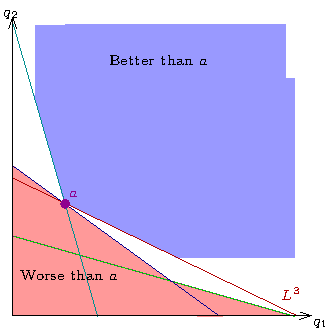
\includegraphics{pics/RevPref7}
\end{center}
The indifference curve through $a$ would have to pass between the blue
and the red shaded areas.
\end{frame}

\begin{frame}
\frametitle{Backing out preferences}
With enough observations we can find the IC. 

\bigskip
\uncover<2->{With fewer observations,
we can approximate it.}\end{frame}

\begin{frame}
\frametitle{Substitution effect}
Suppose you're indifferent between bundles $(q_1,q_2)$ and
$(q_1',q_2')$.
\bigskip

\uncover<2->{
Fix $p_2$ and suppose that you are minimizing cost to stay on that
indifference cost.}
\bigskip

\uncover<3->{At $p_1$ you pick $(q_1,q_2)$. So
\begin{equation}\label{one}
p_1q_1 + p_2q_2 \leq p_1q_1' + p_2q_2'
\end{equation}}

\uncover<4->{At $p_1'$ you pick $(q_1',q_2')$. So
\begin{equation}\label{two}
p_1'q_1' + p_2q_2' \leq p_1'q_1 + p_2q_2
\end{equation}}

\uncover<5->{If you subtract (\ref{two}) from (\ref{one})
\[
(p_1-p_1') (q_1-q_1')\leq 0
\]}

\uncover<6->{This is the law of demand for compensated demand! \\If $p_1 > p_1'$ then
$q_1 < q_1'$ and vice versa.}


\end{frame}

\begin{frame}
\frametitle{Textbook exercise 5.3}
When $Y=1,000$, $p_1=100,$ and $p_2=10$, consumer picks bundle $(q_1,q_2)=(2,80)$.
\bigskip

When $Y'=1,200$, $p_1'=150,$ and $p_2'=10$, consumer picks bundle
$(q_1',q_2')$ where $q_1'=1$.
\bigskip

Can we use revealed preference to determine which of the two bundles the consumer prefers?
\bigskip

\uncover<2->{
Revealed preference: If you pick $x$ when you could have $y$, then you
prefer $x$ to $y$.}

\uncover<3->{\bigskip
Since $p_1'q_1+p_2'q_2=150\times 2+10\times 80 = 1,100 \leq Y'$, the
consumer could afford $(q_1,q_2)$ when he picked $(q_1',q_2')$ he must
prefer $(q_1',q_2')$ to $(q_1,q_2)$.
}
\end{frame}



\end{document}






